\documentclass[14pt]{extbook}
\usepackage{multicol, enumerate, enumitem, hyperref, color, soul, setspace, parskip, fancyhdr} %General Packages
\usepackage{amssymb, amsthm, amsmath, latexsym, units, mathtools} %Math Packages
\everymath{\displaystyle} %All math in Display Style
% Packages with additional options
\usepackage[headsep=0.5cm,headheight=12pt, left=1 in,right= 1 in,top= 1 in,bottom= 1 in]{geometry}
\usepackage[usenames,dvipsnames]{xcolor}
\usepackage{dashrule}  % Package to use the command below to create lines between items
\newcommand{\litem}[1]{\item#1\hspace*{-1cm}\rule{\textwidth}{0.4pt}}
\pagestyle{fancy}
\lhead{Progress Quiz 5}
\chead{}
\rhead{Version ALL}
\lfoot{8497-6012}
\cfoot{}
\rfoot{Summer C 2021}
\begin{document}

\begin{enumerate}
\litem{
Solve the rational equation below. Then, choose the interval(s) that the solution(s) belongs to.\[ \frac{-56}{16x -72} + 1 = \frac{-56}{16x -72} \]\begin{enumerate}[label=\Alph*.]
\item \( x_1 \in [-5.5, -1.5] \text{ and } x_2 \in [2.5,5.5] \)
\item \( x \in [-5.5,-1.5] \)
\item \( x \in [3.5,5.5] \)
\item \( x_1 \in [4.5, 6.5] \text{ and } x_2 \in [2.5,5.5] \)
\item \( \text{All solutions lead to invalid or complex values in the equation.} \)

\end{enumerate} }
\litem{
Choose the equation of the function graphed below.
\begin{center}
    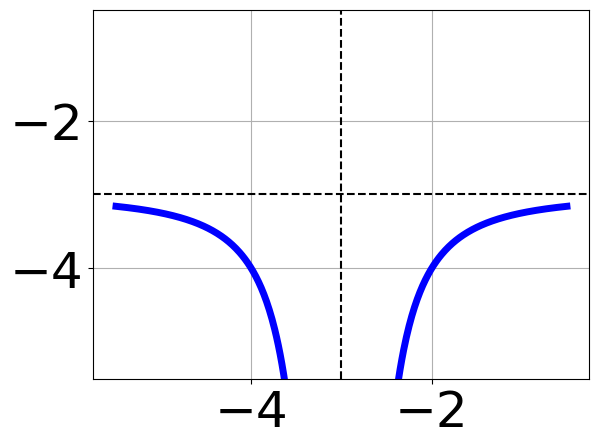
\includegraphics[width=0.5\textwidth]{../Figures/rationalGraphToEquationA.png}
\end{center}
\begin{enumerate}[label=\Alph*.]
\item \( f(x) = \frac{1}{x - 3} - 3 \)
\item \( f(x) = \frac{1}{(x - 3)^2} - 3 \)
\item \( f(x) = \frac{-1}{x + 3} - 3 \)
\item \( f(x) = \frac{-1}{(x + 3)^2} - 3 \)
\item \( \text{None of the above} \)

\end{enumerate} }
\litem{
Choose the equation of the function graphed below.
\begin{center}
    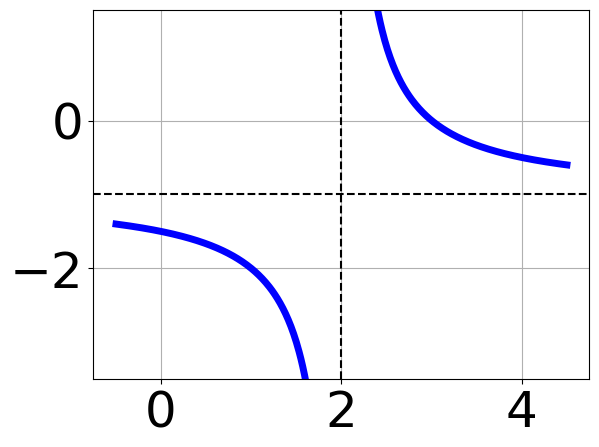
\includegraphics[width=0.5\textwidth]{../Figures/rationalGraphToEquationCopyA.png}
\end{center}
\begin{enumerate}[label=\Alph*.]
\item \( f(x) = \frac{1}{x - 2} - 1 \)
\item \( f(x) = \frac{1}{(x - 2)^2} - 1 \)
\item \( f(x) = \frac{-1}{(x + 2)^2} - 1 \)
\item \( f(x) = \frac{-1}{x + 2} - 1 \)
\item \( \text{None of the above} \)

\end{enumerate} }
\litem{
Choose the graph of the equation below.\[ f(x) = \frac{1}{(x + 3)^2} - 1 \]\begin{enumerate}[label=\Alph*.]
\begin{multicols}{2}\item 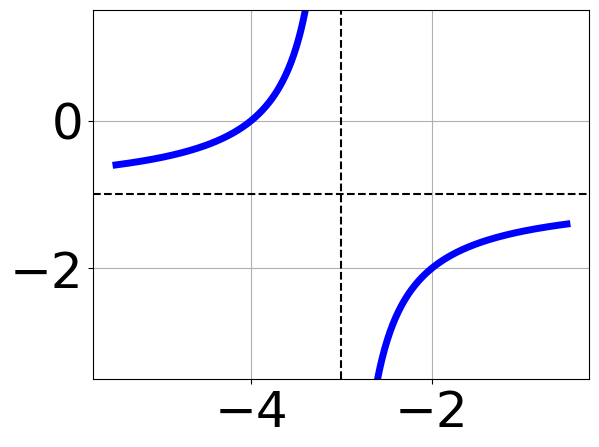
\includegraphics[width = 0.3\textwidth]{../Figures/rationalEquationToGraphCopyAA.png}\item 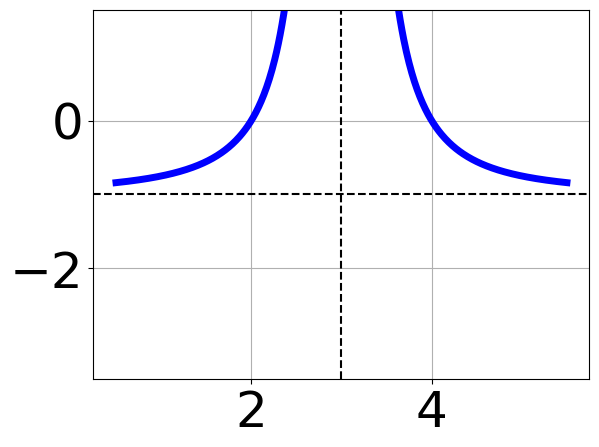
\includegraphics[width = 0.3\textwidth]{../Figures/rationalEquationToGraphCopyBA.png}\item 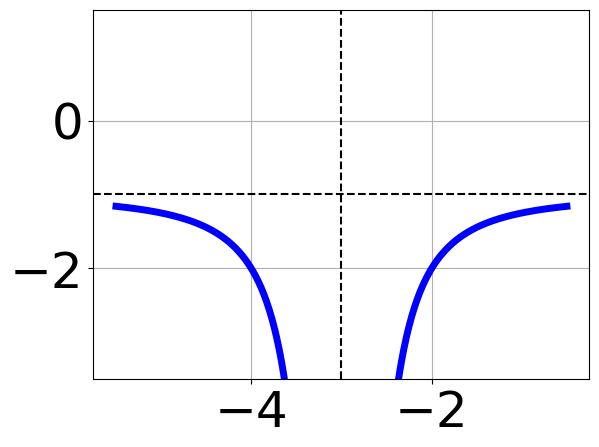
\includegraphics[width = 0.3\textwidth]{../Figures/rationalEquationToGraphCopyCA.png}\item 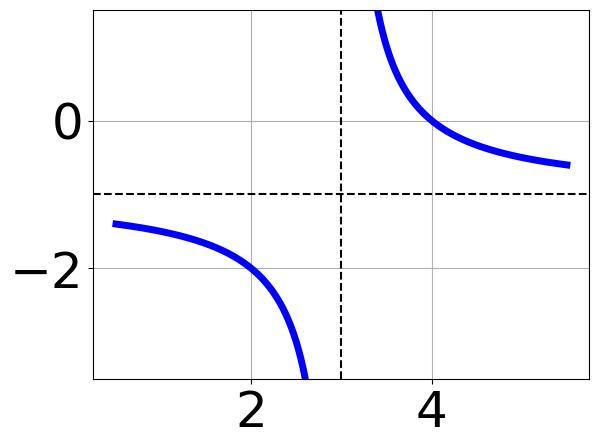
\includegraphics[width = 0.3\textwidth]{../Figures/rationalEquationToGraphCopyDA.png}\end{multicols}\item None of the above.
\end{enumerate} }
\litem{
Solve the rational equation below. Then, choose the interval(s) that the solution(s) belongs to.\[ \frac{-4x}{7x + 6} + \frac{-6x^{2}}{35x^{2} -19 x -42} = \frac{-6}{5x -7} \]\begin{enumerate}[label=\Alph*.]
\item \( x \in [1.53,3.65] \)
\item \( \text{All solutions lead to invalid or complex values in the equation.} \)
\item \( x \in [0.6,1.53] \)
\item \( x_1 \in [-1.34, -0.34] \text{ and } x_2 \in [-3,2.7] \)
\item \( x_1 \in [-1.34, -0.34] \text{ and } x_2 \in [3,6.7] \)

\end{enumerate} }
\litem{
Solve the rational equation below. Then, choose the interval(s) that the solution(s) belongs to.\[ \frac{4x}{4x + 7} + \frac{-2x^{2}}{-8x^{2} +14 x + 49} = \frac{2}{-2x + 7} \]\begin{enumerate}[label=\Alph*.]
\item \( x_1 \in [2.28, 3.46] \text{ and } x_2 \in [-2,3] \)
\item \( x \in [-2.84,-0.99] \)
\item \( x \in [2.68,4.19] \)
\item \( x_1 \in [-2.84, -0.99] \text{ and } x_2 \in [1.5,6.5] \)
\item \( \text{All solutions lead to invalid or complex values in the equation.} \)

\end{enumerate} }
\litem{
Determine the domain of the function below.\[ f(x) = \frac{6}{16x^{2} +40 x + 24} \]\begin{enumerate}[label=\Alph*.]
\item \( \text{All Real numbers except } x = a, \text{ where } a \in [-1.67, -1.4] \)
\item \( \text{All Real numbers except } x = a \text{ and } x = b, \text{ where } a \in [-24.11, -23.87] \text{ and } b \in [-16.78, -15.56] \)
\item \( \text{All Real numbers except } x = a, \text{ where } a \in [-24.11, -23.87] \)
\item \( \text{All Real numbers.} \)
\item \( \text{All Real numbers except } x = a \text{ and } x = b, \text{ where } a \in [-1.67, -1.4] \text{ and } b \in [-1.32, -0.74] \)

\end{enumerate} }
\litem{
Determine the domain of the function below.\[ f(x) = \frac{6}{16x^{2} +8 x -15} \]\begin{enumerate}[label=\Alph*.]
\item \( \text{All Real numbers except } x = a, \text{ where } a \in [-23, -19] \)
\item \( \text{All Real numbers.} \)
\item \( \text{All Real numbers except } x = a, \text{ where } a \in [-4.25, -0.25] \)
\item \( \text{All Real numbers except } x = a \text{ and } x = b, \text{ where } a \in [-23, -19] \text{ and } b \in [12, 13] \)
\item \( \text{All Real numbers except } x = a \text{ and } x = b, \text{ where } a \in [-4.25, -0.25] \text{ and } b \in [0.75, 2.75] \)

\end{enumerate} }
\litem{
Choose the graph of the equation below.\[ f(x) = \frac{-1}{x - 1} + 2 \]\begin{enumerate}[label=\Alph*.]
\begin{multicols}{2}\item 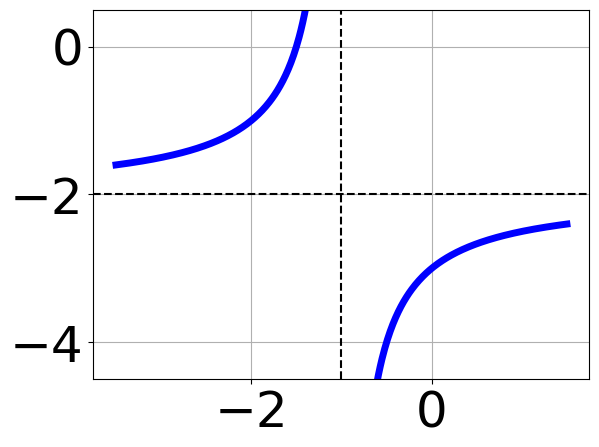
\includegraphics[width = 0.3\textwidth]{../Figures/rationalEquationToGraphAA.png}\item 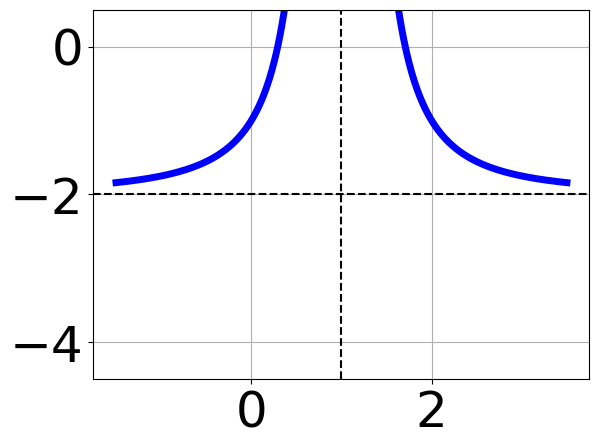
\includegraphics[width = 0.3\textwidth]{../Figures/rationalEquationToGraphBA.png}\item 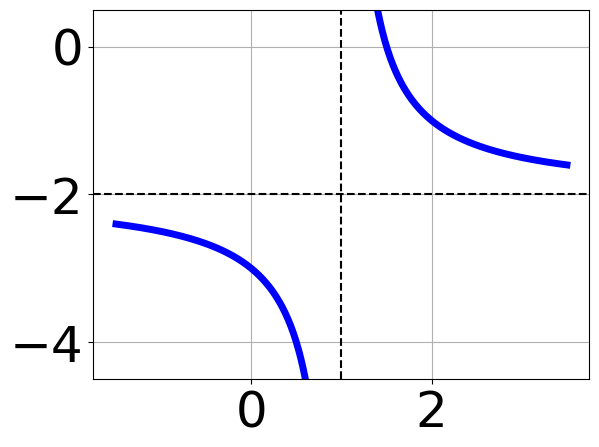
\includegraphics[width = 0.3\textwidth]{../Figures/rationalEquationToGraphCA.png}\item 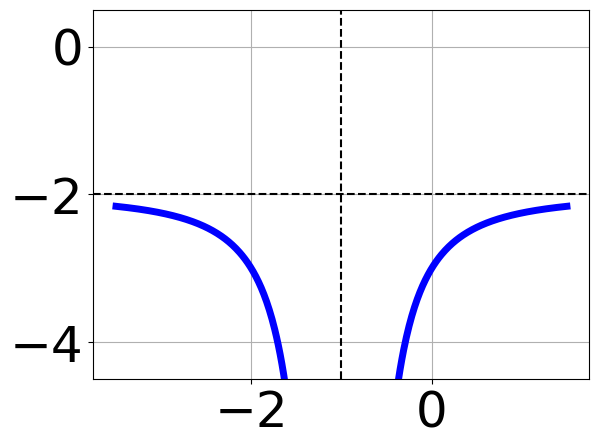
\includegraphics[width = 0.3\textwidth]{../Figures/rationalEquationToGraphDA.png}\end{multicols}\item None of the above.
\end{enumerate} }
\litem{
Solve the rational equation below. Then, choose the interval(s) that the solution(s) belongs to.\[ \frac{108}{72x -36} + 1 = \frac{108}{72x -36} \]\begin{enumerate}[label=\Alph*.]
\item \( x \in [-0.9,-0.2] \)
\item \( x_1 \in [-0.9, -0.2] \text{ and } x_2 \in [-0.5,2.5] \)
\item \( x \in [0.5,2.5] \)
\item \( x_1 \in [0.2, 1.1] \text{ and } x_2 \in [-0.5,2.5] \)
\item \( \text{All solutions lead to invalid or complex values in the equation.} \)

\end{enumerate} }
\litem{
Solve the rational equation below. Then, choose the interval(s) that the solution(s) belongs to.\[ \frac{-20}{70x -40} + 1 = \frac{-20}{70x -40} \]\begin{enumerate}[label=\Alph*.]
\item \( \text{All solutions lead to invalid or complex values in the equation.} \)
\item \( x \in [0.57,1.57] \)
\item \( x_1 \in [0.4, 1.1] \text{ and } x_2 \in [0.57,1.57] \)
\item \( x \in [-1.6,0.3] \)
\item \( x_1 \in [-1.6, 0.3] \text{ and } x_2 \in [0.57,1.57] \)

\end{enumerate} }
\litem{
Choose the equation of the function graphed below.
\begin{center}
    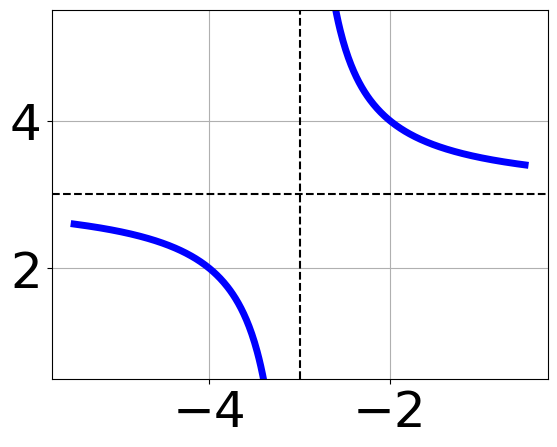
\includegraphics[width=0.5\textwidth]{../Figures/rationalGraphToEquationB.png}
\end{center}
\begin{enumerate}[label=\Alph*.]
\item \( f(x) = \frac{1}{(x + 3)^2} + 3 \)
\item \( f(x) = \frac{-1}{x - 3} + 3 \)
\item \( f(x) = \frac{1}{x + 3} + 3 \)
\item \( f(x) = \frac{-1}{(x - 3)^2} + 3 \)
\item \( \text{None of the above} \)

\end{enumerate} }
\litem{
Choose the equation of the function graphed below.
\begin{center}
    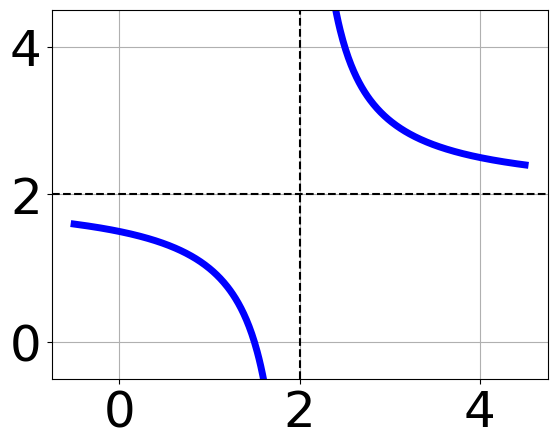
\includegraphics[width=0.5\textwidth]{../Figures/rationalGraphToEquationCopyB.png}
\end{center}
\begin{enumerate}[label=\Alph*.]
\item \( f(x) = \frac{-1}{(x - 2)^2} + 2 \)
\item \( f(x) = \frac{1}{x + 2} + 2 \)
\item \( f(x) = \frac{-1}{x - 2} + 2 \)
\item \( f(x) = \frac{1}{(x + 2)^2} + 2 \)
\item \( \text{None of the above} \)

\end{enumerate} }
\litem{
Choose the graph of the equation below.\[ f(x) = \frac{-1}{(x + 3)^2} + 1 \]\begin{enumerate}[label=\Alph*.]
\begin{multicols}{2}\item 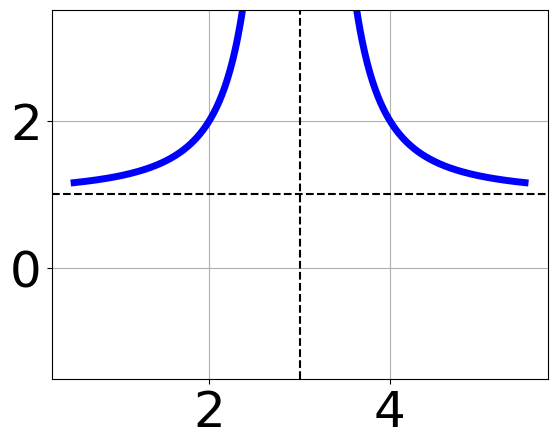
\includegraphics[width = 0.3\textwidth]{../Figures/rationalEquationToGraphCopyAB.png}\item 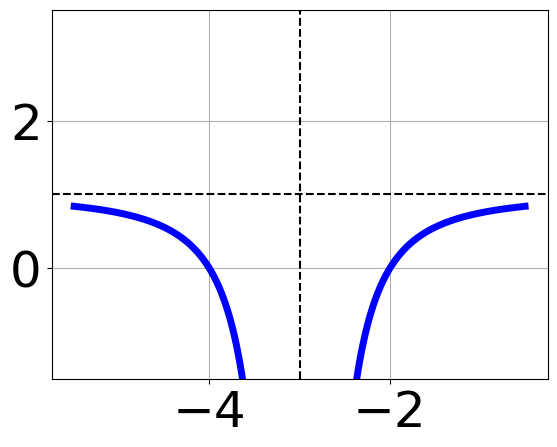
\includegraphics[width = 0.3\textwidth]{../Figures/rationalEquationToGraphCopyBB.png}\item 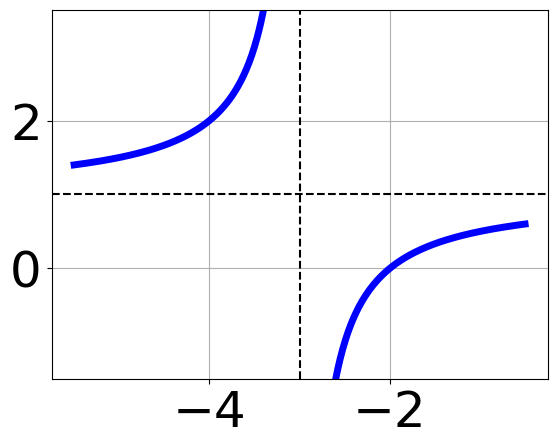
\includegraphics[width = 0.3\textwidth]{../Figures/rationalEquationToGraphCopyCB.png}\item 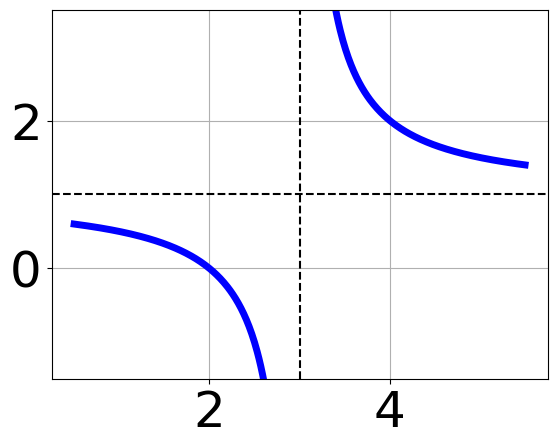
\includegraphics[width = 0.3\textwidth]{../Figures/rationalEquationToGraphCopyDB.png}\end{multicols}\item None of the above.
\end{enumerate} }
\litem{
Solve the rational equation below. Then, choose the interval(s) that the solution(s) belongs to.\[ \frac{-4x}{-5x -5} + \frac{-6x^{2}}{-30x^{2} -60 x -30} = \frac{-2}{6x + 6} \]\begin{enumerate}[label=\Alph*.]
\item \( \text{All solutions lead to invalid or complex values in the equation.} \)
\item \( x \in [-1.37,-0.95] \)
\item \( x_1 \in [-0.62, -0] \text{ and } x_2 \in [-1.92,-1.48] \)
\item \( x_1 \in [-1.37, -0.95] \text{ and } x_2 \in [-1.41,-0.89] \)
\item \( x \in [-1.37,-0.95] \)

\end{enumerate} }
\litem{
Solve the rational equation below. Then, choose the interval(s) that the solution(s) belongs to.\[ \frac{-5x}{-3x -5} + \frac{-4x^{2}}{-9x^{2} -27 x -20} = \frac{-4}{3x + 4} \]\begin{enumerate}[label=\Alph*.]
\item \( x_1 \in [-2.51, -1.62] \text{ and } x_2 \in [-1.47,-1.31] \)
\item \( \text{All solutions lead to invalid or complex values in the equation.} \)
\item \( x_1 \in [-1.11, -0.28] \text{ and } x_2 \in [-2.5,-1.79] \)
\item \( x \in [-1.37,-1.16] \)
\item \( x \in [-2.51,-1.62] \)

\end{enumerate} }
\litem{
Determine the domain of the function below.\[ f(x) = \frac{4}{24x^{2} +30 x + 9} \]\begin{enumerate}[label=\Alph*.]
\item \( \text{All Real numbers except } x = a \text{ and } x = b, \text{ where } a \in [-18.59, -17.66] \text{ and } b \in [-12.34, -11.94] \)
\item \( \text{All Real numbers except } x = a \text{ and } x = b, \text{ where } a \in [-1.29, -0.59] \text{ and } b \in [-0.73, 0.43] \)
\item \( \text{All Real numbers except } x = a, \text{ where } a \in [-18.59, -17.66] \)
\item \( \text{All Real numbers except } x = a, \text{ where } a \in [-1.29, -0.59] \)
\item \( \text{All Real numbers.} \)

\end{enumerate} }
\litem{
Determine the domain of the function below.\[ f(x) = \frac{6}{15x^{2} -35 x + 20} \]\begin{enumerate}[label=\Alph*.]
\item \( \text{All Real numbers except } x = a \text{ and } x = b, \text{ where } a \in [11.97, 12.02] \text{ and } b \in [24.92, 26] \)
\item \( \text{All Real numbers except } x = a \text{ and } x = b, \text{ where } a \in [0.06, 1.24] \text{ and } b \in [1.27, 1.5] \)
\item \( \text{All Real numbers except } x = a, \text{ where } a \in [0.06, 1.24] \)
\item \( \text{All Real numbers except } x = a, \text{ where } a \in [11.97, 12.02] \)
\item \( \text{All Real numbers.} \)

\end{enumerate} }
\litem{
Choose the graph of the equation below.\[ f(x) = \frac{-1}{x - 2} - 1 \]\begin{enumerate}[label=\Alph*.]
\begin{multicols}{2}\item 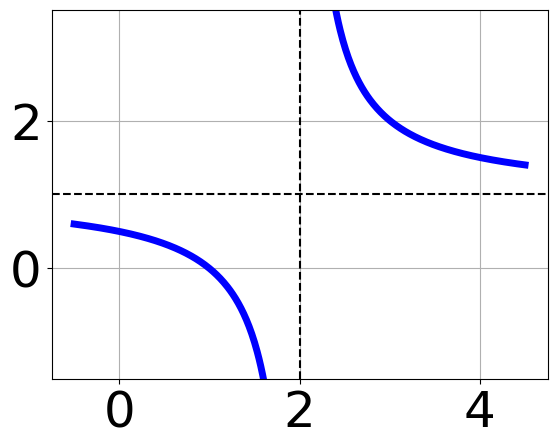
\includegraphics[width = 0.3\textwidth]{../Figures/rationalEquationToGraphAB.png}\item 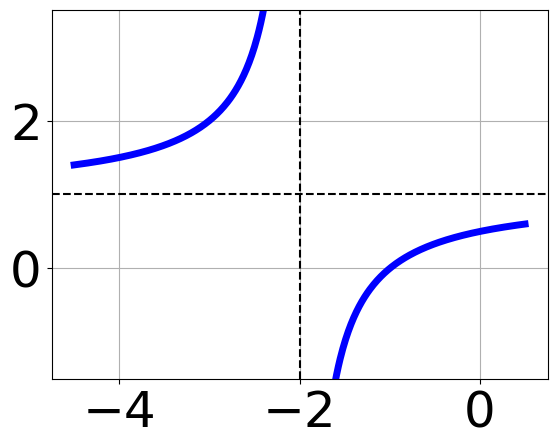
\includegraphics[width = 0.3\textwidth]{../Figures/rationalEquationToGraphBB.png}\item 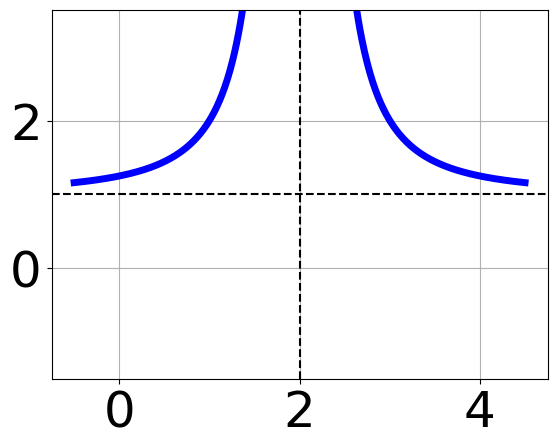
\includegraphics[width = 0.3\textwidth]{../Figures/rationalEquationToGraphCB.png}\item 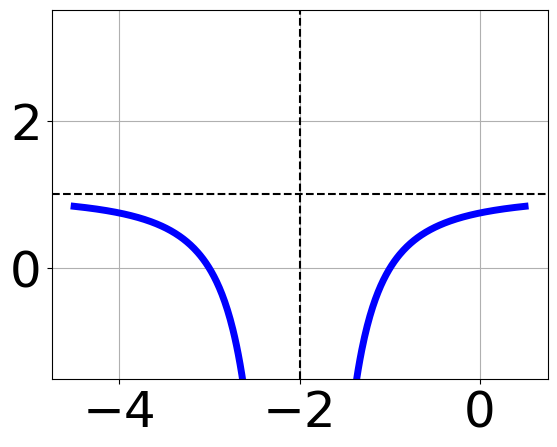
\includegraphics[width = 0.3\textwidth]{../Figures/rationalEquationToGraphDB.png}\end{multicols}\item None of the above.
\end{enumerate} }
\litem{
Solve the rational equation below. Then, choose the interval(s) that the solution(s) belongs to.\[ \frac{-7}{-9x -4} + -6 = \frac{-3}{-36x -16} \]\begin{enumerate}[label=\Alph*.]
\item \( x_1 \in [-0.37, -0.32] \text{ and } x_2 \in [-0.3,1.2] \)
\item \( x \in [0.51,0.59] \)
\item \( \text{All solutions lead to invalid or complex values in the equation.} \)
\item \( x \in [-0.33,1.67] \)
\item \( x_1 \in [-0.42, -0.36] \text{ and } x_2 \in [-1.1,0.3] \)

\end{enumerate} }
\litem{
Solve the rational equation below. Then, choose the interval(s) that the solution(s) belongs to.\[ \frac{5}{7x + 6} + -7 = \frac{-6}{-28x -24} \]\begin{enumerate}[label=\Alph*.]
\item \( x_1 \in [-1.4, -0.7] \text{ and } x_2 \in [0.1,1.6] \)
\item \( \text{All solutions lead to invalid or complex values in the equation.} \)
\item \( x_1 \in [-1.4, -0.7] \text{ and } x_2 \in [-2,0.3] \)
\item \( x \in [-1.79,1.21] \)
\item \( x \in [0.7,2] \)

\end{enumerate} }
\litem{
Choose the equation of the function graphed below.
\begin{center}
    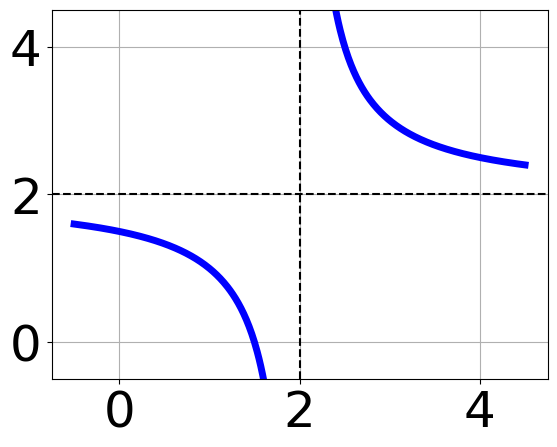
\includegraphics[width=0.5\textwidth]{../Figures/rationalGraphToEquationC.png}
\end{center}
\begin{enumerate}[label=\Alph*.]
\item \( f(x) = \frac{1}{x - 2} + 2 \)
\item \( f(x) = \frac{1}{(x - 2)^2} + 2 \)
\item \( f(x) = \frac{-1}{x + 2} + 2 \)
\item \( f(x) = \frac{-1}{(x + 2)^2} + 2 \)
\item \( \text{None of the above} \)

\end{enumerate} }
\litem{
Choose the equation of the function graphed below.
\begin{center}
    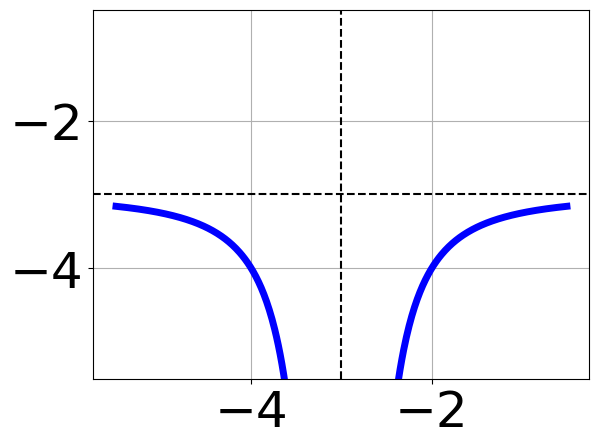
\includegraphics[width=0.5\textwidth]{../Figures/rationalGraphToEquationCopyC.png}
\end{center}
\begin{enumerate}[label=\Alph*.]
\item \( f(x) = \frac{-1}{x + 3} - 3 \)
\item \( f(x) = \frac{1}{(x - 3)^2} - 3 \)
\item \( f(x) = \frac{1}{x - 3} - 3 \)
\item \( f(x) = \frac{-1}{(x + 3)^2} - 3 \)
\item \( \text{None of the above} \)

\end{enumerate} }
\litem{
Choose the graph of the equation below.\[ f(x) = \frac{1}{(x + 1)^2} - 2 \]\begin{enumerate}[label=\Alph*.]
\begin{multicols}{2}\item 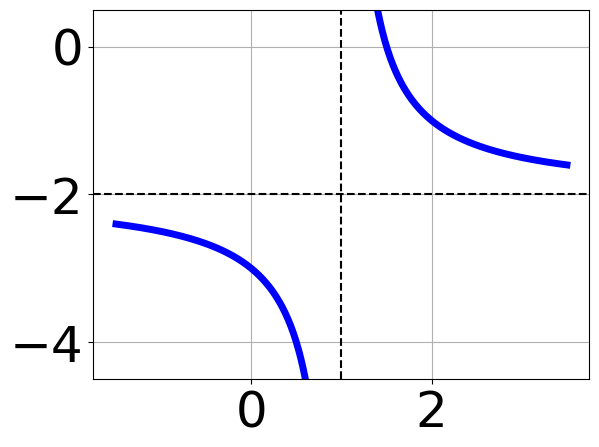
\includegraphics[width = 0.3\textwidth]{../Figures/rationalEquationToGraphCopyAC.png}\item 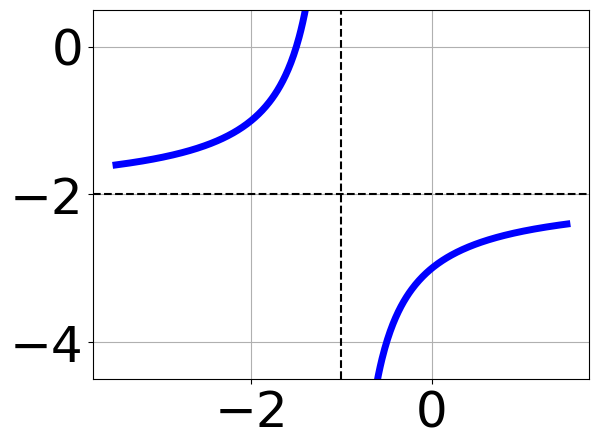
\includegraphics[width = 0.3\textwidth]{../Figures/rationalEquationToGraphCopyBC.png}\item 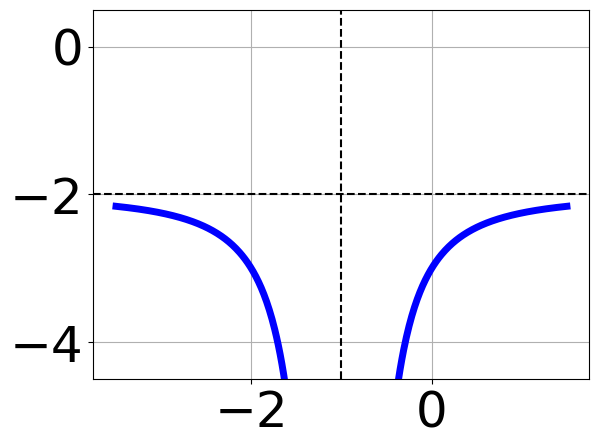
\includegraphics[width = 0.3\textwidth]{../Figures/rationalEquationToGraphCopyCC.png}\item 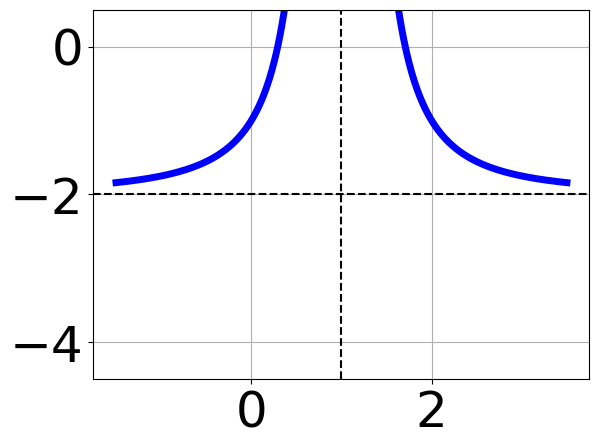
\includegraphics[width = 0.3\textwidth]{../Figures/rationalEquationToGraphCopyDC.png}\end{multicols}\item None of the above.
\end{enumerate} }
\litem{
Solve the rational equation below. Then, choose the interval(s) that the solution(s) belongs to.\[ \frac{-2x}{3x -2} + \frac{-6x^{2}}{6x^{2} +11 x -10} = \frac{-4}{2x + 5} \]\begin{enumerate}[label=\Alph*.]
\item \( \text{All solutions lead to invalid or complex values in the equation.} \)
\item \( x \in [0.65,0.68] \)
\item \( x \in [-2.54,-2.47] \)
\item \( x_1 \in [-2.6, -2.56] \text{ and } x_2 \in [1.56,2.56] \)
\item \( x_1 \in [0.65, 0.68] \text{ and } x_2 \in [-3.5,-1.5] \)

\end{enumerate} }
\litem{
Solve the rational equation below. Then, choose the interval(s) that the solution(s) belongs to.\[ \frac{-3x}{7x + 6} + \frac{-2x^{2}}{-28x^{2} -10 x + 12} = \frac{5}{-4x + 2} \]\begin{enumerate}[label=\Alph*.]
\item \( x_1 \in [-0.99, -0.27] \text{ and } x_2 \in [2.73,11.73] \)
\item \( \text{All solutions lead to invalid or complex values in the equation.} \)
\item \( x \in [0.36,0.75] \)
\item \( x \in [4.07,5.47] \)
\item \( x_1 \in [-0.99, -0.27] \text{ and } x_2 \in [-2.86,2.14] \)

\end{enumerate} }
\litem{
Determine the domain of the function below.\[ f(x) = \frac{6}{18x^{2} -6 x -24} \]\begin{enumerate}[label=\Alph*.]
\item \( \text{All Real numbers except } x = a, \text{ where } a \in [-3, 1] \)
\item \( \text{All Real numbers except } x = a \text{ and } x = b, \text{ where } a \in [-36, -35] \text{ and } b \in [12, 13] \)
\item \( \text{All Real numbers.} \)
\item \( \text{All Real numbers except } x = a, \text{ where } a \in [-36, -35] \)
\item \( \text{All Real numbers except } x = a \text{ and } x = b, \text{ where } a \in [-3, 1] \text{ and } b \in [0.33, 6.33] \)

\end{enumerate} }
\litem{
Determine the domain of the function below.\[ f(x) = \frac{3}{16x^{2} +8 x -24} \]\begin{enumerate}[label=\Alph*.]
\item \( \text{All Real numbers except } x = a \text{ and } x = b, \text{ where } a \in [-25.9, -22.9] \text{ and } b \in [14.9, 16.3] \)
\item \( \text{All Real numbers except } x = a \text{ and } x = b, \text{ where } a \in [-2.5, -0.7] \text{ and } b \in [-0.5, 1.4] \)
\item \( \text{All Real numbers except } x = a, \text{ where } a \in [-2.5, -0.7] \)
\item \( \text{All Real numbers except } x = a, \text{ where } a \in [-25.9, -22.9] \)
\item \( \text{All Real numbers.} \)

\end{enumerate} }
\litem{
Choose the graph of the equation below.\[ f(x) = \frac{-1}{x - 3} - 3 \]\begin{enumerate}[label=\Alph*.]
\begin{multicols}{2}\item 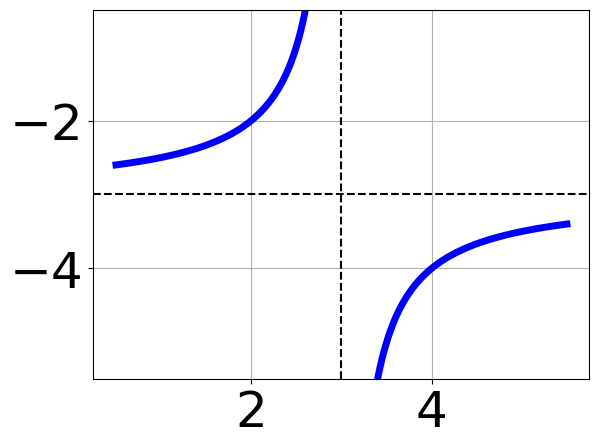
\includegraphics[width = 0.3\textwidth]{../Figures/rationalEquationToGraphAC.png}\item 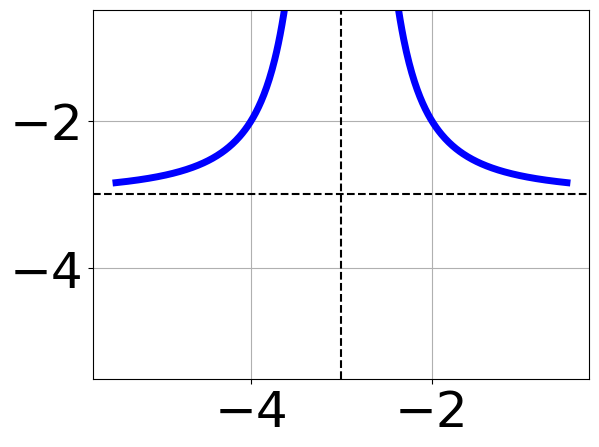
\includegraphics[width = 0.3\textwidth]{../Figures/rationalEquationToGraphBC.png}\item 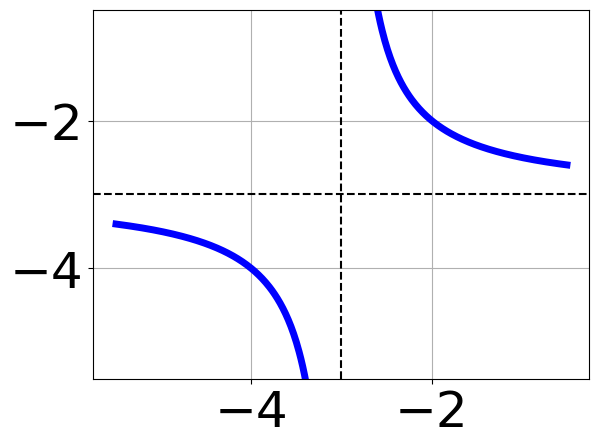
\includegraphics[width = 0.3\textwidth]{../Figures/rationalEquationToGraphCC.png}\item 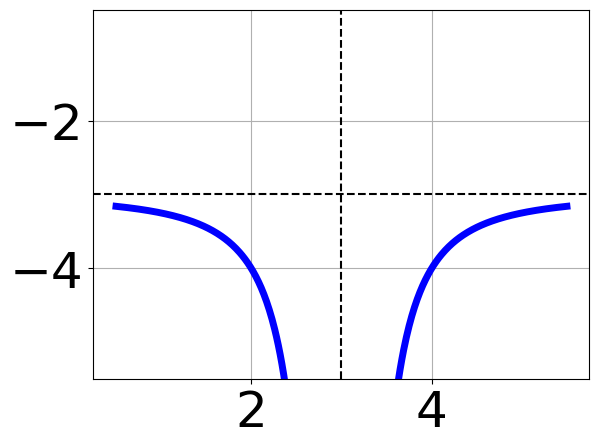
\includegraphics[width = 0.3\textwidth]{../Figures/rationalEquationToGraphDC.png}\end{multicols}\item None of the above.
\end{enumerate} }
\litem{
Solve the rational equation below. Then, choose the interval(s) that the solution(s) belongs to.\[ \frac{88}{88x + 55} + 1 = \frac{88}{88x + 55} \]\begin{enumerate}[label=\Alph*.]
\item \( \text{All solutions lead to invalid or complex values in the equation.} \)
\item \( x \in [-0.62,0.38] \)
\item \( x_1 \in [-1.62, 0.38] \text{ and } x_2 \in [-1.62,0.38] \)
\item \( x_1 \in [-1.62, 0.38] \text{ and } x_2 \in [0.62,1.62] \)
\item \( x \in [-0.38,2.62] \)

\end{enumerate} }
\end{enumerate}

\end{document}